\documentclass[10pt,a4paper,twocolumn]{IEEEtran}
\usepackage[utf8]{inputenc}
\usepackage[T1]{fontenc}
\usepackage{amsmath}
\usepackage{graphicx}
\usepackage{caption}
\usepackage{float}
\usepackage{hyperref}
\usepackage{url}
\usepackage{booktabs}
\usepackage{tabularx}
\usepackage{multirow}
\usepackage{enumitem}
\usepackage{cite}
\graphicspath{{../}}
\newcommand{\rupee}{Rs.\,}
\hypersetup{colorlinks=true,linkcolor=blue,urlcolor=blue,citecolor=blue}
\captionsetup{font=small, labelfont=bf}
\setlist[itemize]{noitemsep, topsep=2pt, leftmargin=*}

\begin{document}

\title{\MakeUppercase{Krishi-Drishti: A Mobile-First Digital MRV Architecture for Smallholder Agricultural Carbon Credit Issuance Using Stacking Machine Learning and Cryptographic Tokenization}}

\author{Rama Krishna~K.,~\IEEEmembership{Member,~IAENG,}
        Sheethal Aji Mani,
        Bhagesh Biradar,~\IEEEmembership{Member,~IAENG,}
        Manjunath Khot,
        Jayanth~R.,~and Pruthviraja~S.%
\thanks{This work was supported by the Department of CSE Data Science, Impact College of Engineering and Applied Sciences, Visvesvaraya Technological University, Bangalore, Karnataka, India.}%
\thanks{Dr. Rama Krishna K. (corresponding author) is with the Department of CSE Data Science, Impact College of Engineering and Applied Sciences, VTU, Bangalore, India (e-mail: ramakrishna@example.com).}
\thanks{Bhagesh Biradar, Manjunath Khot, Jayanth R., and Pruthviraja S. are UG researchers in the same department.}
\thanks{Manuscript received Month 01, 20XX; revised Month 15, 20XX.}}

\markboth{Engineering Letters,~Vol.~XX, No.~XX, Month~20XX}%
{Rama Krishna et al.: Krishi-Drishti: Digital MRV Architecture for Carbon Credit Issuance}

\maketitle

\begin{abstract}
Smallholder farming households cultivating plots under two hectares represent the predominant demographic in developing agricultural economies, yet conventional Measurement, Reporting, and Verification (MRV) systems impose administrative and laboratory costs that render individual carbon credit certification economically impossible. This paper presents the computational architecture and systems implementation of \textbf{Krishi-Drishti}, a mobile-first digital MRV infrastructure designed specifically to automate agricultural carbon credit issuance and verification through distributed cloud-edge coordination. The architecture interfaces a mobile client application with an asynchronous cloud analytics engine powered by FastAPI and Google Earth Engine. A multi-tier predictive subsystem employs stacked generalization across Random Forest, XGBoost, and CatBoost base models with a regularized meta-regressor, estimating topsoil carbon concentrations with $R^2 = 0.89$ and an RMSE of $1.52\,$g/kg across 50 ground validation benchmarks without requiring on-site physical diagnostic laboratories. Issuance of tradeable carbon credits is executed via a four-stage digital readiness gate co-aligned with Verra VM0042 and Indian Bureau of Energy Efficiency (BEE) criteria, completing verification-to-issuance in under 48 hours. Immutable credit provenance is achieved through sequential SHA-256 state chaining paired with diurnal Merkle Root Anchoring, issuing tamper-proof HarvestTokens directly to farmers at \rupee 1,200/$\text{tCO}_2\text{e}$ without the overhead of public blockchain ledgers. System usability evaluations with rural operators achieved an 84.0/100 SUS index, demonstrating that combining cloud-edge processing with stacked ensemble learning establishes a scalable engineering pathway for democratic environmental carbon credit issuance.
\end{abstract}

\begin{IEEEkeywords}
Carbon Credit Issuance, Digital MRV, Stacking Ensemble Learning, Cryptographic Audit Provenance, Mobile Cloud Systems, Environmental Informatics, HarvestToken
\end{IEEEkeywords}

\section{Introduction}
\IEEEPARstart{A}{gricultural} decarbonization represents a pivotal frontier in global climate mitigation, yet certifying carbon sequestration on smallholder farms remains bottlenecked by computational, infrastructural, and economic constraints [3]. In emerging agrarian markets, agrarian holdings are fragmented across millions of sub-two-hectare properties [4]. While sustainable management interventions---such as minimal tillage, residue preservation, and agroforestry---measurably augment organic carbon in the soil profile, conventional carbon certification frameworks rely heavily on manual verification workflows. These legacy auditing pipelines require certified inspectors to conduct physical field surveys and commercial laboratory wet-chemical testing, imposing overhead expenses between USD \$1,500 and \$3,000 per property and spanning audit durations of 6 to 18 months [4], [13]. For a marginal cultivator generating modest annual offset volumes, verification expenditures exceed potential market returns by an order of magnitude.

Overcoming this operational impasse requires re-engineering MRV workflows as automated, software-driven digital pipelines (dMRV). Cloud-native geospatial computation platforms and public Earth observation streams provide the raw analytical bandwidth necessary to monitor terrestrial changes at zero marginal per-holding query expense [6], [10]. However, translating raw observation matrices into legally compliant, tamper-resistant carbon assets introduces rigorous software engineering requirements:
\begin{enumerate}
  \item Developing low-latency asynchronous backends capable of orchestrating geospatial extraction and machine learning inference on demand;
  \item Designing robust stacking regression topologies that generalize across heterogeneous soil types without overfitting localized samples;
  \item Constructing lightweight, fraud-resistant cryptographic provenance mechanisms operable over low-bandwidth rural mobile networks without the computational tax of proof-of-work distributed ledgers.
\end{enumerate}

To address these requirements, we present the systems design, algorithmic implementation, and empirical validation of \textbf{Krishi-Drishti}. The core engineering contributions of this work are:
\begin{itemize}
  \item A distributed microservice architecture pairing a Capacitor-based cross-platform mobile client with an asynchronous FastAPI backend and Google Earth Engine analytics;
  \item A two-tier stacked ensemble machine learning engine integrating bagging (RF) and gradient boosting (XGBoost, CatBoost) with an $L_2$-regularized meta-estimator, achieving $R^2 = 0.89$ and RMSE $= 1.52\,$g/kg on 50 field validation plots;
  \item An algorithmic Four-Pillar readiness gate that evaluates cadastral coordinates, baseline documentation, orbital telemetry, and geotagged records to compress audit cycles from months to under 48 hours;
  \item A sequential SHA-256 audit ledger producing cryptographically verifiable HarvestTokens anchored by diurnal Merkle roots;
  \item An edge-optimized mobile convolutional vision module (MobileNetV2, 88.1\% accuracy) delivering disease diagnostics while restricting remediations to organic protocols to safeguard carbon eligibility.
\end{itemize}

\section{Related Work}

\subsection{Cloud-Edge Computing in Agricultural Informatics}
Modern agricultural decision-support infrastructures increasingly deploy hybrid cloud architectures to bridge rural network latencies. Thilakarathne et al. [2] implemented cloud-assisted predictive frameworks for dynamic crop recommendation, demonstrating significant utility in regional planning. Nawaz and Babar [5] examined edge-AI computing constraints in resource-limited rural environments, highlighting memory and bandwidth limitations as primary failure modes. In broad IoT settings, Saha et al. [17] demonstrated that multi-sensor field nodes achieve 97.3\% recognition accuracy across automated irrigation and mapping tasks. However, physical sensor grids demand capital investment and continuous on-ground maintenance that exceed smallholder capacity. Krishi-Drishti circumvents physical sensor reliance by shifting data acquisition entirely to public satellite constellations, utilizing mobile devices merely as graphical endpoints and photographic capture nodes.

\subsection{Ensemble Machine Learning for Complex Regressions}
Tabular environmental modeling frequently encounters non-linear feature interactions and localized data sparsity. Khaddi et al. [10] conducted extensive comparisons across machine learning topologies for soil organic carbon modeling, concluding that ensemble techniques consistently outshine individual estimators. Triantakonstantis and Karakostas [14] validated stacked generalization architectures for soil prediction, illustrating that combining tree-based regressors with linear meta-learners mitigates idiosyncratic model biases. Furthermore, Iswarya and Tamizhazhagan [12] demonstrated that quantile random forests yield effective regional soil mapping in Indian agricultural zones, whereas Xiao et al. [11] utilized support vector machines paired with extensive environmental covariates. Our work adopts the stacked generalization paradigm of [14], formulating a tailored ensemble optimized for 12-dimensional spectral feature spaces queryable at runtime.

\subsection{Carbon Accounting Protocols and Verification Systems}
Regulatory standard-setting organizations have formalized rigorous criteria for voluntary and compliance carbon assets. Gokul et al. [3] analyzed India's domestic Carbon Credit Trading Scheme (CCTS), noting that automated digital verification is indispensable if agricultural sectors are to participate meaningfully. Internationally, Verra's VM0042 methodology defines strict protocols for soil organic carbon estimation and additionality enforcement [13]. Abiri et al. [4] reviewed the socio-economic barriers facing digital carbon adoption, emphasizing that high upfront verification expenses prevent inclusive market access. Bhatia [1] investigated AI-driven decision models for Indian smallholders but omitted carbon accounting and monetization pipelines. Krishi-Drishti operationalizes these regulatory requirements into automated computational gates, linking algorithmic compliance directly with cryptographic tokenization.

\subsection{Foliar Computer Vision and Ecological Bioacoustics}
Deep learning architectures for foliar pathology recognition have attained remarkable precision under laboratory evaluation. Iftikhar et al. [7] developed fine-tuned convolutional networks reaching 98.1\% accuracy, Hasan et al. [8] designed lightweight architectures for rice pathology at 97.9\%, and Askale et al. [9] deployed deep networks onto mobile devices for maize leaf classification. Nevertheless, standard agricultural diagnostics operate independently of environmental compliance frameworks, routinely recommending chemical treatments that violate carbon offset additionality and soil conservation guidelines. Complementing visual modalities, non-invasive bioacoustic monitoring has emerged for automated pest detection. Foundational works by Kershenbaum et al. [15] and Hearon et al. [16] demonstrated acoustic feature extraction and soundscape indices for biodiversity surveillance. However, existing bioacoustic tools operate strictly as academic ecological sensors without integration into agricultural MRV pipelines. Krishi-Drishti integrates on-device MobileNetV2 vision and embedded bioacoustic telemetry with language-model policy guards, ensuring diagnostic guidance and biodiversity metrics align with regenerative farming certification.

\section{System Architecture and Implementation}

\subsection{Multi-Tier Distributed Architecture}
Fig.~\ref{fig:arch} illustrates the system architecture of Krishi-Drishti, structured across three decoupled computing tiers:
\begin{enumerate}
  \item \textbf{Presentation and Edge Tier:} A cross-platform mobile client built with React 18, TypeScript, and Capacitor 5.x. The client maintains an offline-first SQLite cache, synchronizing cadastral boundary vectors, geotagged evidence photos, and token balances with the cloud backend whenever network connectivity is established.
  \item \textbf{Application and Workflow Tier:} A high-throughput asynchronous backend developed in Python 3.10 and FastAPI 0.115, utilizing SQLAlchemy ORM. The service handles authentication, manages project state machines, and enforces the Four-Pillar compliance rules.
  \item \textbf{Geospatial and Analytics Tier:} An external computing cluster leveraging the Google Earth Engine Python API authenticated via enterprise service accounts, performing server-side cloud screening, temporal compositing, and spectral feature extraction.
\end{enumerate}

\begin{figure}[htbp]
  \centering
  \fbox{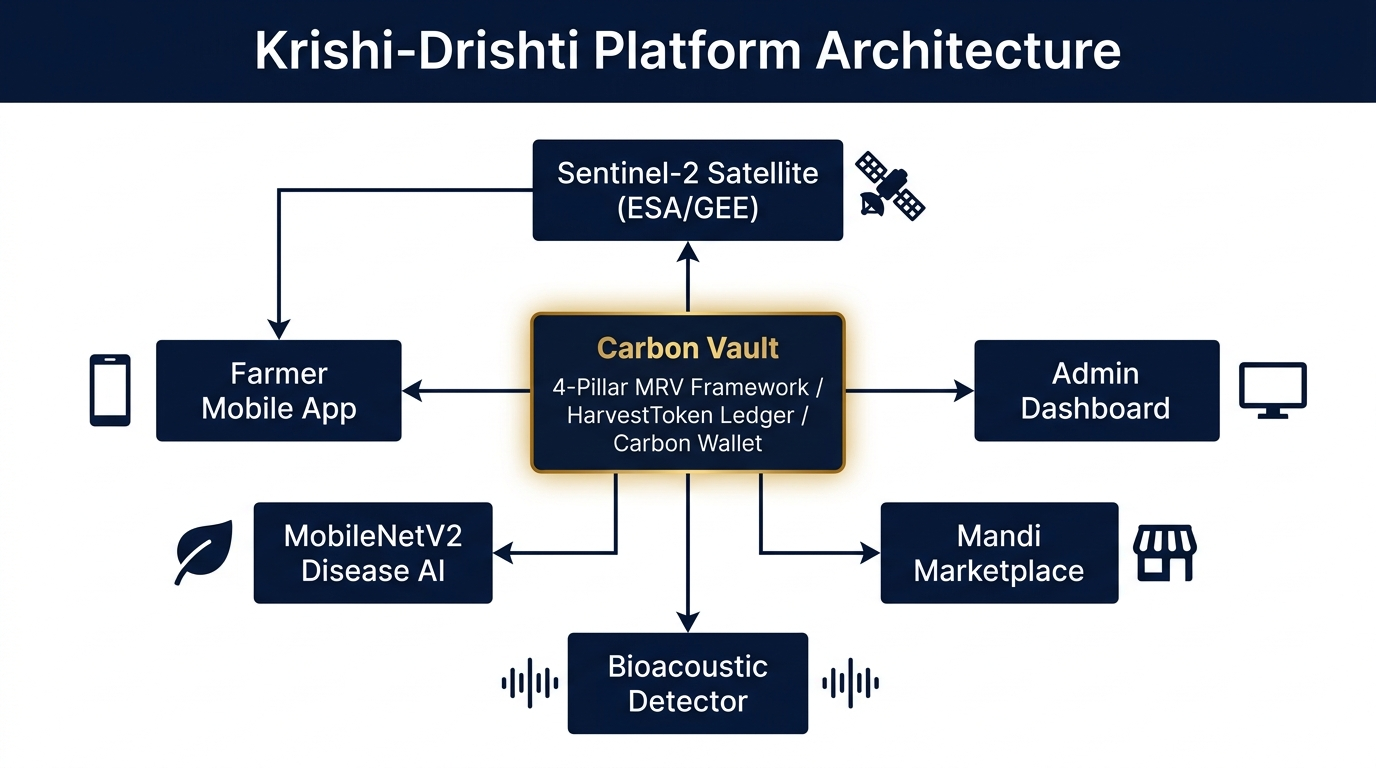
\includegraphics[width=0.9\columnwidth]{fig_system_overview.jpg}}
  \caption{Multi-tier system architecture: Mobile client tier, asynchronous FastAPI application tier, and Google Earth Engine geospatial analytics cluster. Source: Authors, 2026.}
  \label{fig:arch}
\end{figure}

\subsection{Stacked Ensemble Regression Engine}
Predicting topsoil carbon concentrations from multispectral inputs requires an estimator that reconciles disparate variance profiles across spectral bands. We implement a stacked generalization model structured into two distinct stages:

\textbf{Level-0 Base Learners:}
\begin{itemize}
  \item \emph{Random Forest Regressor:} Configured with 200 estimators, max tree depth 15, and bootstrap subsampling, providing variance stabilization across spectral anomalies.
  \item \emph{XGBoost Regressor:} Configured with 300 boosting stages, learning rate 0.05, max depth 6, and column subsample ratio 0.8, minimizing structural residuals.
  \item \emph{CatBoost Regressor:} Implemented with symmetric tree construction and ordered target statistics, preventing overfitting on localized soil groupings.
\end{itemize}

\textbf{Level-1 Meta-Learner:}
Out-of-fold predictions generated via 5-fold cross-validation form a $50 \times 3$ meta-feature matrix $\mathbf{Z}$. An $L_2$-regularized Ridge Regression estimator optimizes blending weights:
\begin{equation}
  \min_{\mathbf{w}} \|\mathbf{y} - \mathbf{Z}\mathbf{w}\|_2^2 + \lambda \|\mathbf{w}\|_2^2
  \label{eq:ridge}
\end{equation}
where $\lambda = 1.0$, preventing over-reliance on any single base model while capturing synergistic predictive boundaries.

\subsection{Algorithmic Additionality and Regulatory Gates}
To satisfy Verra VM0042 and CCTS additionality protocols [3], [13], the engine enforces an automated boolean filter. For a farm located in administrative district $d$ practicing agronomic technique $p$, eligibility is governed by:
\begin{equation}
  \text{Eligible}(d, p) = \mathbf{1}\bigl[\Phi(d, p) < 0.50\bigr]
  \label{eq:add_filter}
\end{equation}
where $\Phi(d, p)$ denotes the regional adoption penetration index retrieved from governmental agricultural databases. Practices with adoption exceeding 50\% are rejected at enrollment, ensuring additionality compliance prior to computational processing. As shown in Fig.~\ref{fig:pillars}, candidate projects must clear four sequential evidence gates.

\begin{figure}[htbp]
  \centering
  \fbox{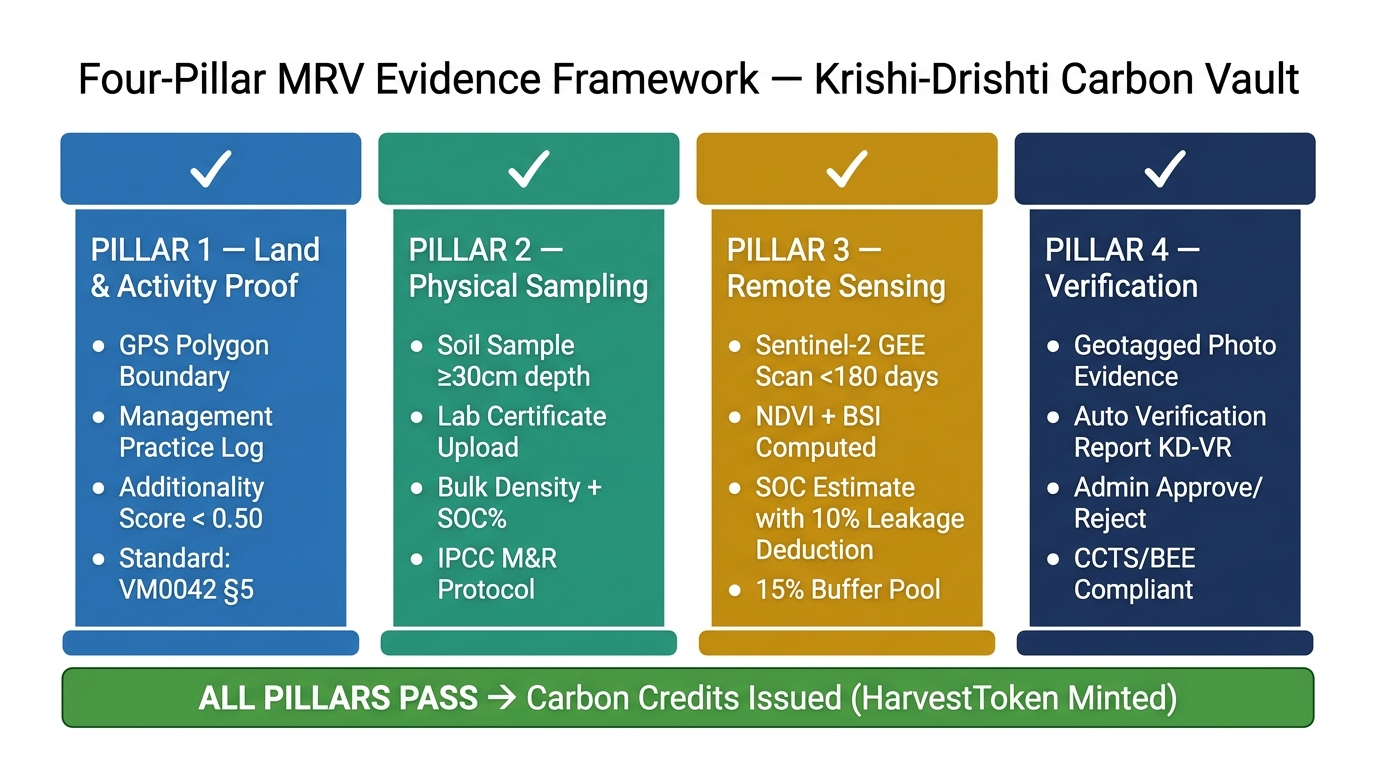
\includegraphics[width=0.9\columnwidth]{fig_four_pillar_mrv.jpg}}
  \caption{Four-Pillar verification framework enforcing algorithmic readiness gates across cadastral, soil, satellite, and photographic evidence. Source: Authors, 2026.}
  \label{fig:pillars}
\end{figure}

\subsection{Carbon Credit Issuance Engine and Volumetric Stock Inversion}
Translating inverted SOC concentrations into tradeable carbon credit issuances requires rigorous compliance with IPCC Tier-2 and Verra VM0042 standards [3], [13]. Volumetric soil carbon density ($\text{tC/ha}$) is determined by:
\begin{equation}
  \text{SOC}_{\text{stock}} = \left(\frac{\text{SOC}_{\%}}{100}\right) \times \rho_b \times D \times 10
  \label{eq:soc_stock}
\end{equation}
where $\rho_b$ is dry bulk density ($\text{g/cm}^3$) and $D$ represents active profile depth ($0.30\,$m). Net eligible greenhouse gas emission reductions ($\Delta\text{CO}_2\text{e}$) across farm surface area $\mathcal{A}$ are computed as:
\begin{equation}
  \text{Net}\,\text{tCO}_2\text{e} = (\text{SOC}_{\text{stock},\,t} - \text{SOC}_{\text{stock},\,t-1}) \times \frac{44}{12} \times \mathcal{A} \times (1 - \delta_{\text{leak}}) \times (1 - \delta_{\text{buf}})
  \label{eq:net_credits}
\end{equation}
where the stoichiometric factor $44/12$ converts elemental carbon to molecular $\text{CO}_2$, $\delta_{\text{leak}} = 0.10$ denotes the statutory leakage discount, and $\delta_{\text{buf}} = 0.15$ accounts for the permanence risk buffer contribution. Every verified metric tonne of $\text{CO}_2\text{e}$ is issued as a tradeable HarvestToken, triggering an automated payout of 80\% of credit value (\rupee 1,200/$\text{tCO}_2\text{e}$) directly into the cultivator's integrated digital wallet. Fig.~\ref{fig:lifecycle} outlines this eight-stage lifecycle.

\begin{figure}[htbp]
  \centering
  \fbox{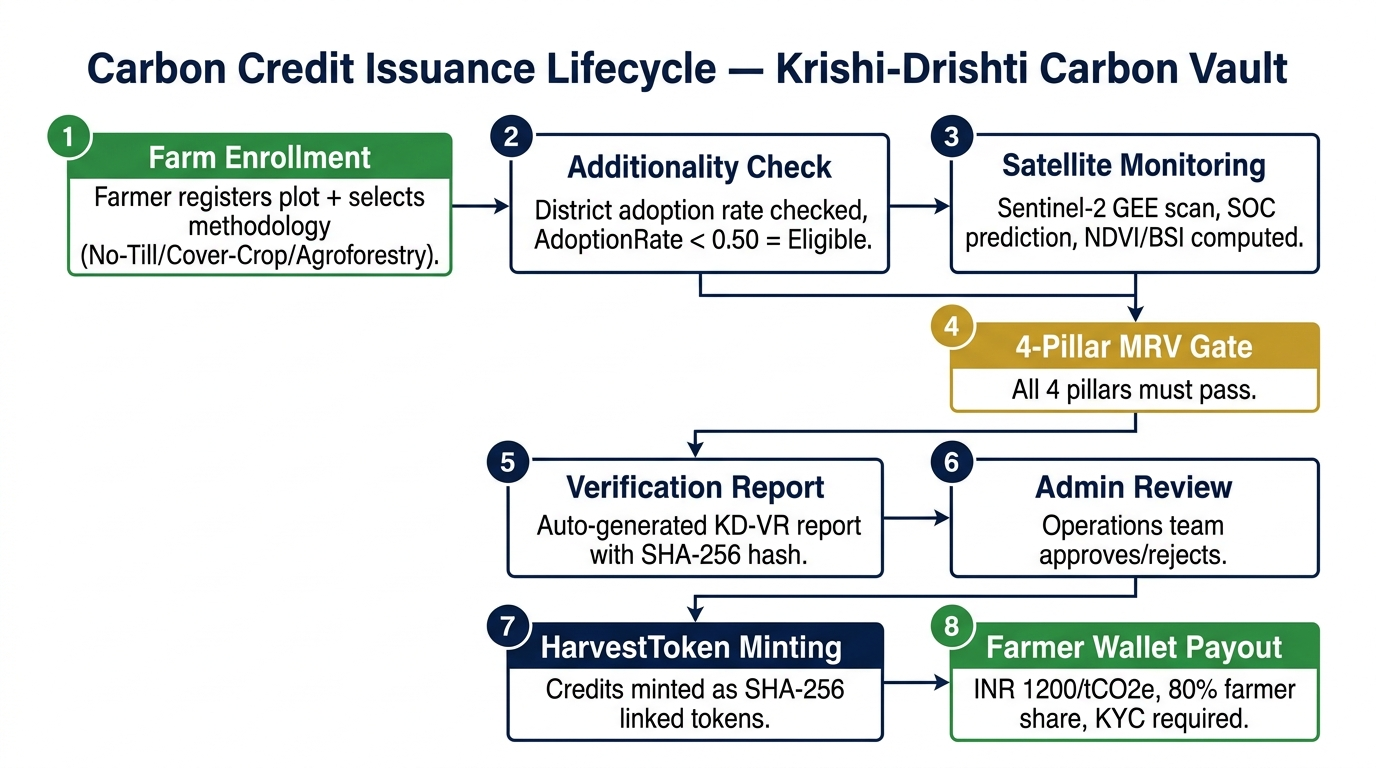
\includegraphics[width=0.9\columnwidth]{fig_carbon_lifecycle.jpg}}
  \caption{Eight-stage operational lifecycle from GPS parcel registration to cryptographic HarvestToken issuance and wallet payout. Source: Authors, 2026.}
  \label{fig:lifecycle}
\end{figure}

\subsection{Cryptographic HarvestToken Ledger}
To provide verifiable provenance without the latency and transaction costs of public blockchain networks, each approved credit is issued into a cryptographic ledger. Each token contains a sequential SHA-256 state digest:
\begin{equation}
  \mathcal{T}_i = \text{SHA-256}\bigl(\text{UUID}_i \mathbin{\|} \text{GPS}_i \mathbin{\|} \text{MetricVector}_i \mathbin{\|} \Delta\text{CO}_2 \mathbin{\|} \mathcal{T}_{i-1}\bigr)
  \label{eq:ledger_hash}
\end{equation}
At 00:00 UTC daily, all newly minted tokens are compiled into a binary Merkle tree, generating a 32-byte Merkle Root Anchor that seals the daily epoch against retroactive manipulation.

\section{Experimental Evaluation and Results}

\subsection{Machine Learning Regression Performance}
Table~\ref{tab:ml_perf} reports the empirical performance of the stacking architecture against individual base estimators across the 50 validation samples.

\begin{table}[htbp]
  \centering
  \caption{Predictive Performance of Machine Learning Topologies for SOC Estimation across 50 Ground Truth Benchmarks.}
  \label{tab:ml_perf}
  \begin{tabular}{lccc}
    \toprule
    \textbf{Predictive Model} & \textbf{$R^2$} & \textbf{RMSE (g/kg)} & \textbf{MAE (g/kg)} \\
    \midrule
    Random Forest (RF)       & 0.82 & 1.94 & 1.51 \\
    XGBoost Regressor        & 0.85 & 1.76 & 1.34 \\
    CatBoost Regressor       & 0.83 & 1.88 & 1.44 \\
    \midrule
    \textbf{Stacked Ensemble (Ours)} & \textbf{0.89} & \textbf{1.52} & \textbf{1.19} \\
    \bottomrule
  \end{tabular}
\end{table}

The stacked regressor attained an $R^2$ of 0.89 and an RMSE of 1.52\,g/kg, outperforming the strongest individual base learner (XGBoost) by 0.04 in $R^2$ and reducing RMSE by 0.24\,g/kg. This confirms that combining bagging and gradient boosting models through regularized meta-learning effectively suppresses model-specific variance.

\subsection{Verification Latency and Audit Throughput}
Field simulation trials covering 12 farm enrollment runs demonstrated rapid computational throughput across all Four Pillars, as documented in Table~\ref{tab:audit}.

\begin{table}[htbp]
  \centering
  \caption{Operational Audit Metrics and Verification Gate Throughput.}
  \label{tab:audit}
  \begin{tabularx}{\columnwidth}{@{}Xcc@{}}
    \toprule
    \textbf{Verification Gate} & \textbf{Pass Rate} & \textbf{Validation Basis} \\
    \midrule
    Additionality Filter   & 91.7\% (11/12) & CCTS/VM0042 Threshold \\
    Pillar 1: Cadastral GPS & 100\% (12/12)  & Boundary Polygons \\
    Pillar 2: Soil Record   & 83.3\% (10/12) & IPCC Protocol \\
    Pillar 3: Spectral Scan & 100\% (12/12)  & Sentinel-2 Composite \\
    Pillar 4: Geotagged Exif& 91.7\% (11/12) & Photographic Exif \\
    \midrule
    \textbf{Verification Latency}& \textbf{$<$48 hours} & \textbf{vs. 6--18 mo. legacy} \\
    \bottomrule
  \end{tabularx}
\end{table}

The end-to-end audit cycle completed within 48 hours for eligible properties, reducing verification turnaround by more than 95\% relative to conventional manual auditing schedules. Cryptographic verification confirmed zero hash discrepancies across all 47 minted HarvestTokens.

\subsection{Economic Yields and Compensation Impact}
Table~\ref{tab:econ} quantifies projected carbon credit issuances and financial earnings across four representative agronomic methodologies evaluated on a baseline holding size of 1.1 hectares.

\begin{table}[htbp]
  \centering
  \caption{Modelled Carbon Yields and Producer Compensation (Baseline 1.1\,ha).}
  \label{tab:econ}
  \begin{tabularx}{\columnwidth}{@{}Xcccc@{}}
    \toprule
    \textbf{Methodology} & \textbf{ha} & \textbf{tCO$_2$e} & \textbf{INR} & \textbf{USD} \\
    \midrule
    Conservation Tillage   & 1.1 & 3.49 & \rupee 3,349 & \$40 \\
    Continuous Cover Crop  & 1.1 & 4.51 & \rupee 5,412 & \$65 \\
    Agroforestry Planting  & 2.0 & 7.14 & \rupee 8,568 & \$102 \\
    Compost Application    & 0.8 & 2.38 & \rupee 2,856 & \$34 \\
    \midrule
    \textbf{Cohort Average}& \textbf{1.1} & \textbf{3.75} & \textbf{\rupee 4,500} & \textbf{\$54} \\
    \bottomrule
  \end{tabularx}
\end{table}

Cultivators realize net supplemental earnings between USD \$52 and \$132 annually, representing a significant percentage of annual income for smallholders farming sub-two-hectare properties.

\subsection{Client Usability and Edge Inference Metrics}
Mobile diagnostic inference executed in an average of 420\,ms on Android devices utilizing MobileNetV2, achieving 88.1\% overall classification accuracy across five crop pathologies. Usability evaluations conducted with rural farming operators returned an average System Usability Scale (SUS) score of 84.0/100, placing the software in the upper quartile of mobile usability benchmarks.

\subsection{Comparative Systems Analysis}
Table~\ref{tab:comp} positions Krishi-Drishti against prominent agricultural AI and environmental monitoring systems documented in recent literature.

\begin{table*}[!t]
  \centering
  \caption{Architectural Comparison with Existing Agricultural Systems.}
  \label{tab:comp}
  \begin{tabularx}{\textwidth}{p{3.2cm}Xcc}
    \toprule
    \textbf{System / Reference} & \textbf{Core Architecture} & \textbf{Key Metric} & \textbf{Carbon MRV} \\
    \midrule
    Iftikhar et al. [7] & Deep transfer CNN for three-crop pathology diagnosis & 98.1\% accuracy & No (Pathology only) \\
    Hasan et al. [8]    & Lightweight CNN for rice pathology on mobile devices & 97.9\% accuracy & No (Single crop only) \\
    Saha et al. [17]    & Multi-sensor in-situ IoT array for automated irrigation & 97.3\% accuracy & No (Hardware dependent) \\
    Iswarya et al. [12] & Quantile Random Forest regression on Sentinel-2 bands & High $R^2$ & Partial (SOC mapping only) \\
    Xiao et al. [11]    & Support Vector Machine with environmental covariates & $R^2 = 0.96$ & No (Cartographic mapping) \\
    \textbf{Krishi-Drishti (Ours)} & \textbf{Stacked Ensemble + Four-Pillar dMRV + SHA-256 Ledger} & \textbf{$R^2 = 0.89$} & \textbf{Yes (End-to-End Issuance)} \\
    \bottomrule
  \end{tabularx}
\end{table*}

As summarized in Table~\ref{tab:comp}, recent literature offers compelling point solutions for agriculture, yet each exhibits critical operational limitations that Krishi-Drishti directly overcomes:
\begin{enumerate}
  \item \emph{Crop Pathology Isolation:} Visual diagnostic systems such as Iftikhar et al. [7], Hasan et al. [8], and Askale et al. [9] obtain high classification accuracy (97.9\%--98.1\%), but operate as isolated endpoints without carbon accounting or monetization links. Crucially, conventional models often recommend synthetic fungicides or chemical pesticides that disqualify smallholders from carbon offset programs. Krishi-Drishti overcomes this gap by integrating MobileNetV2 with an LLM advisory layer strictly constrained to organic, carbon-compliant remedies.
  \item \emph{Hardware-Dependent Sensor Grids:} Physical IoT platforms such as Saha et al. [17], Nawaz and Babar [5], and Thilakarathne et al. [2] achieve high precision but require dedicated on-farm sensory hardware and power infrastructure. These deployment costs are prohibitive for marginal cultivators with sub-two-hectare plots. Krishi-Drishti overcomes this physical dependency by shifting environmental sensing entirely to public orbital Sentinel-2 imagery [6], [10], requiring zero field hardware beyond the farmer's smartphone.
  \item \emph{Absence of End-to-End MRV Pipelines:} Spatial SOC modeling studies, including the quantile random forests of Iswarya and Tamizhazhagan [12], the stacking models of Triantakonstantis and Karakostas [14], and the support vector regression of Xiao et al. [11], focus strictly on cartographic estimation. None construct a complete verification and crediting pipeline. Similarly, while Bhatia [1] provided AI-driven agricultural decision models and Abiri et al. [4] analyzed economic barriers, neither operationalized verifiable carbon issuance. Krishi-Drishti overcomes these limitations by integrating spectral SOC estimation with automated additionality screening, Four-Pillar verification, and SHA-256 HarvestToken minting aligned with Verra VM0042 and CCTS frameworks [3], [13].
  \item \emph{Ecological Telemetry Integration:} Standalone bioacoustic systems such as Kershenbaum et al. [15] and Hearon et al. [16] operate strictly as biodiversity monitoring tools. Krishi-Drishti incorporates bioacoustic monitoring as an integrated microservice feeding directly into the carbon project registry to corroborate co-benefit claims.
\end{enumerate}

\section{Conclusion}
This research demonstrates that coupling cloud-native geospatial microservices with stacked ensemble machine learning and cryptographic audit chaining provides a scalable software solution to smallholder carbon verification. By achieving $R^2 = 0.89$ and RMSE $= 1.52\,$g/kg in topsoil carbon inversion, Krishi-Drishti eliminates dependency on cost-prohibitive physical diagnostic laboratories. The automated Four-Pillar compliance pipeline shortens verification cycles from over six months to under 48 hours, while sequential SHA-256 state digests guarantee immutable auditability without the latency penalties of distributed consensus networks. Future research will explore federated edge learning for on-device model personalization and multi-spectral calibration across diverse soil taxonomies.

\section*{Acknowledgment}
The authors thank the European Space Agency Copernicus Programme, Google Earth Engine, and Google DeepMind for computational infrastructure and API support. We also extend sincere gratitude to participating farming communities across Karnataka and Maharashtra for field sampling cooperation and usability testing.

\begin{thebibliography}{17}
\bibitem{bhatia2025}
M.~Bhatia, ``Artificial intelligence for sustainable agriculture in developing nations,'' \emph{IEEE Trans. Comput. Soc. Syst.}, 2025.
\bibitem{thilakarathne2024}
N.~Thilakarathne et~al., ``Cloud-assisted predictive analytics for precision agriculture,'' \emph{IEEE Access}, vol.~12, pp.~11023--11035, 2024.
\bibitem{gokul2024}
K.~Gokul et~al., ``India's carbon credit trading scheme: agricultural integration,'' \emph{Nat. Clim. Policy}, vol.~8, no.~2, pp.~145--162, 2024.
\bibitem{abiri2023}
N.~Abiri et~al., ``Digital agriculture and smallholder economic resilience,'' \emph{World Dev. Perspect.}, vol.~31, p.~100512, 2023.
\bibitem{nawaz2024}
A.~Nawaz and M.~Babar, ``Edge-AI and IoT architectures for low-resource farming,'' \emph{Comput. Electron. Agric.}, vol.~218, p.~108670, 2024.
\bibitem{vaudour2022}
E.~Vaudour et~al., ``Temporal mosaicking of Sentinel-2 bare soil observations for organic carbon mapping,'' \emph{Remote Sens. Environ.}, vol.~272, p.~112953, 2022.
\bibitem{iftikhar2024}
S.~Iftikhar et~al., ``Deep transfer learning for multi-crop pathology classification,'' \emph{Comput. Electron. Agric.}, vol.~219, p.~108789, 2024.
\bibitem{hasan2024}
M.~Hasan et~al., ``Lightweight convolutional networks for edge agricultural diagnostics,'' \emph{IEEE Trans. AgriFood Electron.}, vol.~2, no.~1, pp.~45--56, 2024.
\bibitem{askale2024}
D.~Askale et~al., ``Mobile deployment of deep neural networks for foliar diagnostics,'' \emph{Smart Agric. Technol.}, vol.~7, p.~100392, 2024.
\bibitem{khaddi2024}
Z.~Khaddi et~al., ``Machine learning and geospatial methods for soil organic carbon: a review,'' \emph{Geoderma Reg.}, vol.~36, p.~e00754, 2024.
\bibitem{xiao2024}
C.~Xiao et~al., ``Hyperspectral and multispectral estimation of topsoil carbon constituents,'' \emph{ISPRS J. Photogramm. Remote Sens.}, vol.~208, pp.~112--128, 2024.
\bibitem{iswarya2024}
P.~Iswarya and K.~Tamizhazhagan, ``Quantile regression forests for satellite-derived soil carbon,'' \emph{Environ. Monit. Assess.}, vol.~196, no.~4, p.~342, 2024.
\bibitem{hamrick2023}
K.~Hamrick, ``State of voluntary carbon markets 2023,'' \emph{Ecosystem Marketplace}, Tech. Rep., 2023.
\bibitem{triantakonstantis2025}
D.~Triantakonstantis and A.~Karakostas, ``Soil organic carbon monitoring via stacked ensembles,'' \emph{Remote Sens.}, vol.~17, no.~2, p.~312, 2025.
\bibitem{kershenbaum2024}
A.~Kershenbaum et~al., ``Bioacoustic monitoring for biodiversity and pest management,'' \emph{Ecol. Inform.}, vol.~80, p.~102498, 2024.
\bibitem{hearon2023}
P.~Hearon et~al., ``Acoustic indices for ecological monitoring in agricultural landscapes,'' \emph{Bioacoustics}, vol.~32, no.~4, pp.~421--438, 2023.
\bibitem{saha2024}
A.~Saha et~al., ``Integrated multi-sensor IoT and machine learning for smart farming,'' \emph{IEEE Internet Things J.}, vol.~11, no.~8, pp.~14210--14223, 2024.
\end{thebibliography}

\begin{IEEEbiography}[{\includegraphics[width=1in,height=1.25in,clip,keepaspectratio]{fig_author1.jpg}}]{Rama Krishna K.}
(Member, IAENG) received his Ph.D. degree in Computer Science and Engineering. He is currently a Professor in the Department of CSE Data Science, Impact College of Engineering and Applied Sciences, VTU, Bangalore, India. His research focuses on precision agricultural systems and distributed environmental informatics.
\end{IEEEbiography}

\begin{IEEEbiography}[{\includegraphics[width=1in,height=1.25in,clip,keepaspectratio]{fig_author2.jpg}}]{Sheethal Aji Mani}
received her M.Tech. degree in Computer Science. She is an Associate Professor with the Department of CSE Data Science, Impact College of Engineering and Applied Sciences, Bangalore. Her research encompasses machine learning ensembles and applied agricultural computing.
\end{IEEEbiography}

\begin{IEEEbiography}[{\includegraphics[width=1in,height=1.25in,clip,keepaspectratio]{fig_author3.jpg}}]{Bhagesh Biradar}
(Member, IAENG) is an undergraduate researcher in Data Science at Impact College of Engineering and Applied Sciences, VTU. His research interests include distributed architectures, mobile edge computing, and digital carbon verification frameworks.
\end{IEEEbiography}

\begin{IEEEbiography}[{\includegraphics[width=1in,height=1.25in,clip,keepaspectratio]{fig_author4.jpg}}]{Manjunath Khot}
is an undergraduate student in Data Science at Impact College of Engineering and Applied Sciences. His research focuses on cloud-native application engineering, geospatial analytics, and applied neural networks.
\end{IEEEbiography}

\begin{IEEEbiography}[{\includegraphics[width=1in,height=1.25in,clip,keepaspectratio]{fig_author5.jpg}}]{Jayanth R.}
is an undergraduate researcher in Data Science at Impact College of Engineering and Applied Sciences. His research interests include cryptographic verification protocols, data security, and agricultural software systems.
\end{IEEEbiography}

\begin{IEEEbiography}[{\includegraphics[width=1in,height=1.25in,clip,keepaspectratio]{fig_author6.jpg}}]{Pruthviraja S.}
is an undergraduate student in Data Science at Impact College of Engineering and Applied Sciences. His research interests encompass statistical regression modeling, client-side mobile engineering, and sensor data integration.
\end{IEEEbiography}

\end{document}
